\documentclass[11pt ,a4paper , twoside , openright ]{article}
\usepackage{layouts}
\usepackage[T1]{fontenc}
\usepackage[utf8]{inputenc}
\usepackage{lmodern}
\usepackage{hyperref}
\usepackage[a4paper,top=3cm,bottom=3cm,left=2.5cm,right=2.5cm]{geometry}
\usepackage[square,numbers]{natbib}
\bibliographystyle{abbrvnat}
\usepackage[italian]{babel}
\usepackage[usenames]{color} 
\usepackage{listings} 
\usepackage{color}
\usepackage{graphicx}
\usepackage[bottom]{footmisc}
\graphicspath{ {./images/} }
\definecolor{mygreen}{rgb}{0,0.6,0}
\definecolor{mygray}{rgb}{0.5,0.5,0.5}
\definecolor{mymauve}{rgb}{0.58,0,0.82}
\usepackage{tikz} % for background logo in frontespizio
\addtolength{\skip\footins}{3pc plus 5pt}
\renewcommand{\arraystretch}{1.5}
\pagestyle{plain}
\usepackage{comment}



\lstset{ 
	backgroundcolor=\color{white}, 
	basicstyle=\footnotesize,
	breakatwhitespace=false, 
	breaklines=true,
	captionpos=b, 
	commentstyle=\color{mygreen}, 
	escapeinside={\%*}{*)}, 
	extendedchars=true, 
	frame=single,
	keepspaces=true, 
	keywordstyle=\color{blue},
	morekeywords={*,...}, 
	numbers=left, 
	numbersep=5pt, 
	numberstyle=\tiny\color{mygray}, 
	rulecolor=\color{black}, 
	showspaces=false, 
	showstringspaces=false, 
	showtabs=false, 
	stepnumber=1, 
	stringstyle=\color{mymauve}, 
	tabsize=2, 
}

\definecolor{darkgray}{rgb}{.4,.4,.4}
\definecolor{purple}{rgb}{0.65, 0.12, 0.82}

\lstdefinelanguage{JavaScript}{
	keywords={typeof, new, true, false, catch, function, return, null, catch, switch, var, if, in, while, do, else, case, break},
	keywordstyle=\color{blue}\bfseries,
	ndkeywords={class, export, boolean, throw, implements, import, this},
	ndkeywordstyle=\color{darkgray}\bfseries,
	identifierstyle=\color{black},
	sensitive=false,
	comment=[l]{//},
	morecomment=[s]{/*}{*/},
	commentstyle=\color{purple}\ttfamily,
	stringstyle=\color{red}\ttfamily,
	morestring=[b]',
	morestring=[b]"
}

\lstset{
	language=JavaScript,
	extendedchars=true,
	basicstyle=\small\ttfamily,
	showstringspaces=false,
	showspaces=false,
	numbers=left,
	numberstyle=\scriptsize,
	numbersep=9pt,
	tabsize=2,
	breaklines=true,
	showtabs=false,
	captionpos=b
}

\author{
	Daniele Rigon - 857319 \\
}


\pagestyle{plain}
\author{Daniele Rigon}
\title{Tesi}
\makeindex
\usepackage{titlesec}

\titleformat{\chapter}[display]
{\Huge\bfseries}{}{0pt}{\thechapter.\ }
\titleformat{name=\chapter,numberless}[display]
{\Huge\bfseries}{}{0pt}{}

\begin{document}
	\thispagestyle{empty}
	\begin{tikzpicture}[remember picture,overlay]
	\node[inner sep=0pt,anchor=0,opacity=0.5]{
\includegraphics{CaFoscariLogo.png}};
	\node[inner sep=40pt,anchor=45,opacity=0.5]{Universit\'a};
	\node[inner sep=55pt,anchor=55,opacity=0.5]{Ca' Foscari};
	\node[inner sep=70pt,anchor=56,opacity=0.5]{Venezia};
	\end{tikzpicture}
	\begin{center}
		\vspace*{0.5cm}
		\Large
		\LARGE \textbf{Corso di Laurea }\\
		\LARGE \textbf{in Informatica}\\
		\textit{\large Ordinamento ex D.M. 270/2004}
		
		\vspace*{1cm}
		\Large Tesi di Laurea\\
		
		\vspace*{1cm}
		\LARGE \textbf{Web APIs Security}\\
	\end{center}
	\begin{flushleft}
		\vspace*{2.6cm} \normalsize
		\textbf{Relatore}\\
		Dott. Stefano Calzavara
		
		\vspace*{1.3cm} \normalsize
		\textbf{Correlatore}\\
		Dott. Marco Squarcina
				
		\vspace*{1.3cm} \normalsize
		\textbf{Laureando}\\
		Daniele Rigon \\
		Matricola 857319 \\		
		
		\vspace*{1.3cm} \normalsize
		\textbf{Anno Accademico}\\
		2018/2019 \\	
	\end{flushleft}

\pagebreak
\cleardoublepage
\tableofcontents

\newpage
\section{Introduzione}
Negli ultimi decenni il World Wide Web è diventanto sempre più presente nella quotidianità di ogni individuo e, come la maggior parte delle cose, presenta aspetti positivi e negativi;
essendo il web un mondo vastissimo, sono numerosi i rischi presenti al suo interno.
\\
L'obiettivo di questa tesi è spiegare i problemi di sicurezza legati alle APIs Web prendendo come threat model un Web attacker il quale può avere due differenti scenari: il primo, più semplice, è un sito web personale nel quale immettiamo le informazioni, per quanto riguarda la PaymentRequest API \cite{rif1}, o accettiamo di condividere la nostra posizione nel caso della Geolocation API \cite{rif2}; il secondo scenario mostra come un Web attacker possa aggiungere propri contenuti all'interno di pagine web esterne al proprio sito riuscendo comunque a rubare informazioni sensibili.
\\
Le API sono delle interfacce che gli sviluppatori e i programmatori possono utilizzare per espandere le funzionalità di programmi o applicazioni, ad esempio facendo interagire due programmi, o due piattaforme, o un programma e una piattaforma, che altrimenti sarebbero state incompatibili.
Un esempio sono le API di Google Maps, messe a disposizione di tutti gli sviluppatori che le volessero utilizzare per un loro programma o piattaforma web, ad esempio per realizzare mappe personalizzate o per integrarle in siti web per servizi di ricerca georeferenziati o usarle all'interno di applicazioni per smartphone e/o tablet.
Un altro esempio sono le API di Facebook, le quali danno la possibilità agli sviluppatori di usare alcune delle proprie funzionalità per realizzare delle applicazioni da usare poi all'interno del social network, facilitando di molto la programmazione delle nuove app o funzionalità.
\\
Queste API facilitano di molto la programmazione e sono utili nell'integrazione di piattaforme differenti tra loro, ma presentano anche delle vulnerabilità.
\\
Questo problema viene studiato nella tesi prendendo in esame un piccolo set di API, mostrando come siano state trovate delle vulnerabilità di sicurezza e privacy all'interno di queste sottolineando come possano venire rubate da un web attacker le informazioni sensibili degli utenti ed essere usate poi da terzi.
\\
La tesi si divide in tre parti corrispondenti alle tre API prese in esame. 
\\
La prima è la Geolocation API la quale, utilizzata nei siti web o nelle web app, serve a tracciare la posizione dell'utente, con possibili rischi di problemi di privacy poichè un Web attacker potrebbe tracciare la posizione dell'utente e rubarla.
\\
La seconda API studiata è la PaymentRequest API, la quale salva le informazioni dell'utente, sia personali che di pagamento, cosi da poterle riutilizzare automaticamente senza doverle reinserirle ogni qualvolta se ne ha bisogno, mostrando però che queste possono essere intercettate e rubate da un Web attacker.
\\
L'ultimo argomento preso in esame, che è anche il più complesso, riguarda i Service Worker \cite{rif3}, i quali vengono usati principalmente per il caching in modo da migliorare l'esperienza utente, mostrando però anche come questi possano essere utilizzati in modo malevolo per rubare informazioni dell'utente intercettando le richieste di rete.
\\
Tutto il codice presente nella tesi è reperibile al seguente repository GitHub \url{https://github.com/danielerigon4/Tesi-Web-Api}.
\cleardoublepage


\section{Geolocation}
\subsection{Overview}
La Geolocation API viene utilizzata per ottenere la posizione geografica di un utente. 
Poiché questo può compromettere la privacy la posizione non è disponibile a meno che l'utente non la approvi: su un dispositivo mobile avremo un set di coordinate provenienti dal sensore GPS mentre su un portatile potremo usare il posizionamento legato all’ip della connessione internet.
\subsection{Specifiche}

\subsubsection{Oggetto della geolocalizzazione}
Nella Geolocation API la posizione viene resa nota utilizzando la proprietà \textit{navigator.geolocation} \cite{rif4} presente nell'oggetto \textit{Navigator}, un'interfaccia che rappresenta lo stato dell'utente. Se l'oggetto esiste, il servizio di geolocalizzazione è disponibile. Per testare l'esistenza di tale oggetto, così da avere disponibili i metodi di geolocalizzazione, bisogna verificare se l'oggetto esiste, nel modo:
\lstinputlisting{code/GeolocationInNavigator.js}

\subsubsection{Metodi}
Ci sono solamente tre metodi a disposizione: \textit{getCurrentPosition}, \textit{watchPosition} e \textit{clearWatch}. I primi due sono utili a ottenere la posizione corrente mentre il terzo serve ad annullare la ricerca della posizione corrente. 
La differenza tra i primi due va ricercata nella loro periodicità, mentre il primo metodo fornisce il dato una sola volta, il secondo si attiva automaticamente ogni qualvolta la posizione cambi, o ogni tot intervallo di tempo.
\\
La sintassi per invocare questi metodi è la seguente:
\lstinputlisting{code/Sintassi.js}
dove è obbligatoria solamente la callback in caso di successo \textit{success}, mentre gli altri due parametri sono opzionali.
\\
La \textit{successCallback} viene chiamata quando vi è un'operazione di successo alla chiamata di una nuova posizione.
La \textit{errorCallback} viene chiamata quando vi sono uno o più errori, e vengono gestiti all'interno di questo metodo.
\textit{Options} definisce i parametri in base ai quali vengono poi chiamate le callback di successo o fallimento.
Un esempio concreto, preso da \cite{rif5}, è questo:
\pagebreak
\lstinputlisting{code/metodiGeolocation.js} 


\textbf{GetCurrentPosition}
\\
Il metodo \textit{GetCuttentPosition} viene chiamato per ottenere la posizione corrente dell'utente, fornendo il dato ogni volta che viene chiamata.

\textbf{WatchPosition}
\\
Il metodo \textit{WatchPosition} restituisce la posizione dell'utente ad ogni intervallo di tempo specificato.

\textbf{ClearWatch}
\\
Il metodo \textit{clearWatch} viene chiamato per annullare il monitoraggio della posizione dell'utente.
\newpage
Un esempio \cite{rif8} dell'uso di questi metodi è il seguente: \\
\lstinputlisting{code/EsempioCompleto.js}
Che produrrà la seguente pagina:
\begin{figure}[h]
	\centering
	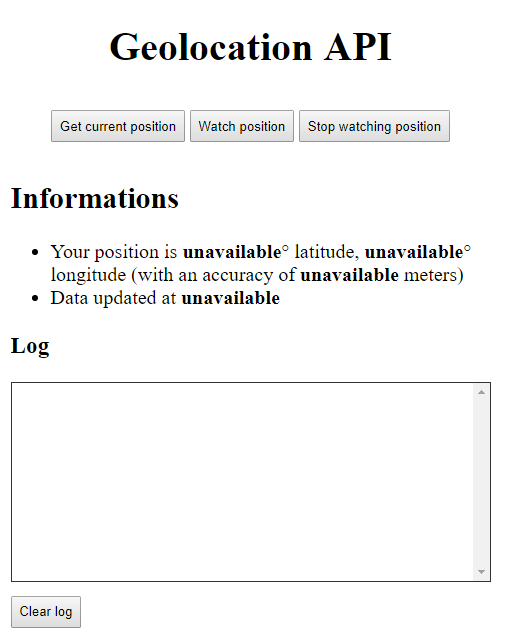
\includegraphics[width=0.5\linewidth]{geo1}
	\caption{Pagina info Geolocation}
	\label{fig: Pagina info Geolocation}
\end{figure}
\pagebreak
\\
Quando saranno chiamati i metodi getCurrentposition o WatchPosition verrà chiesto all'utente il permesso per usare la posizione.
\begin{figure}[h]
	\centering
	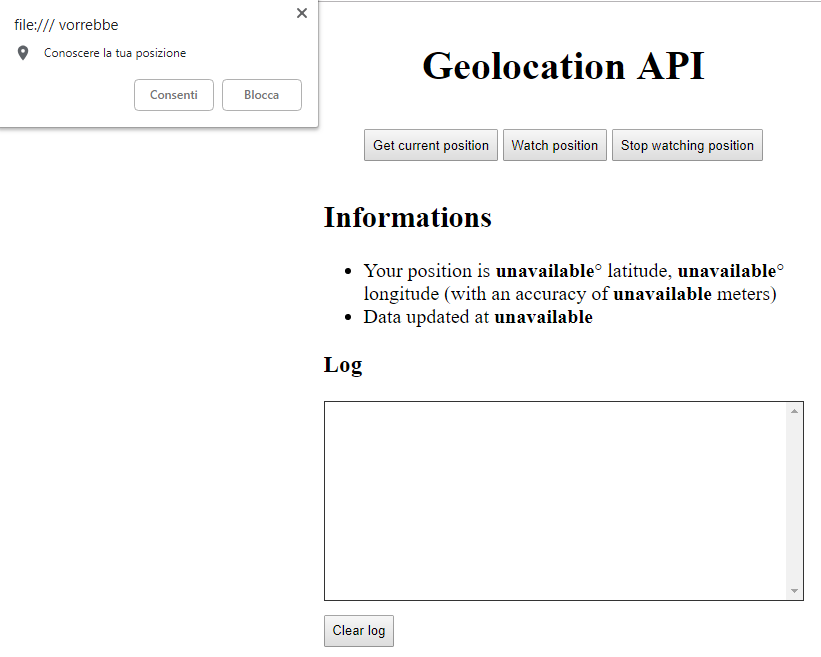
\includegraphics[width=0.4\linewidth]{geo2}
	\caption{Richiesta permesso}
	\label{fig: Richiesta permesso}
\end{figure}
\\
Se l'utente rifiuta la posizione non viene calcolata e viene mostrato un messaggio di errore in console.
\begin{figure}[h]
	\centering
	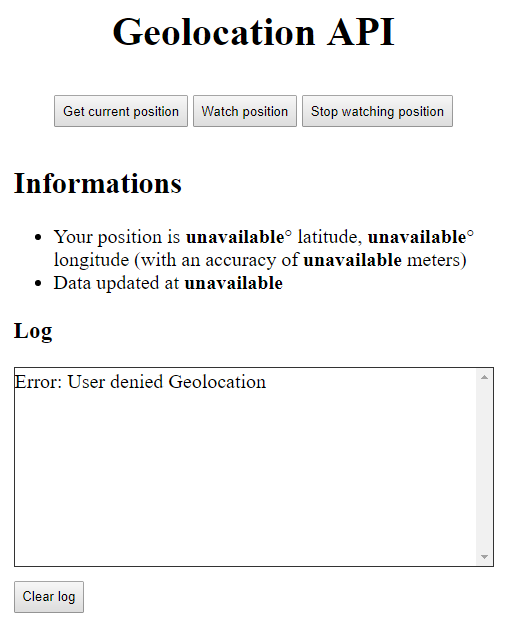
\includegraphics[width=0.4\linewidth]{geo3}
	\caption{Rifiuto autorizzazione}
	\label{fig: Rifiuto autorizzazione}
\end{figure}
\pagebreak
\\
Se l'utente acconsente all'utilizzo della posizione verrà mostrato un messaggio di conferma in console e saranno mostrate a video tutte le informazioni disponibili dell'utente.
\begin{figure}[h]
	\centering
	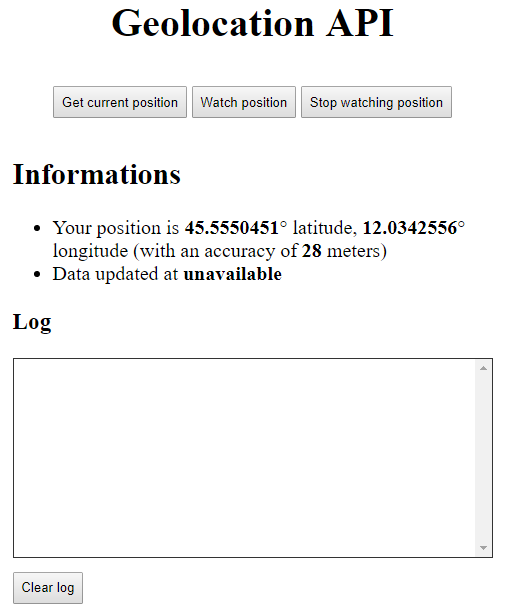
\includegraphics[width=0.4\linewidth]{geo4}
	\caption{Accetto autorizzazione}
	\label{fig: Accetto autorizzazione}
\end{figure}
\\


\subsection{Problemi sicurezza/privacy} 
Uno dei principali problemi della Geolocation API \cite{rif6} \cite{rif7} è rappresentato dal fatto che un Web Attacker può rubare la posizione ad un utente che accetta di condividerla all'interno del sito attaccante ignaro del fatto che non sia sicuro, oppure attraverso un cross-site scripting (XSS) \footnote{Tipo di vulnerabilità di sicurezza presente nelle applicazioni web. Questo attacco consente agli aggressori di inserire script sul lato client in pagine Web visualizzate da altri utenti, e questa vulnerabilità può essere usata dagli aggressori per bypassare i controlli di accesso, come ad esempio la same origin policy.} all'interno di un sito che considerato fidato. Gli oggetti per tracciare le coordinate (latitudine e longitudine) risiedono all'interno del DOM il quale è accessibile con JavaScript e attraverso il quale si possono prendere le informazioni sulla posizione dell'utente. 
Nella maggior parte dei casi succede che la posizione viene richiesta e condivisa in quanto viene chiesta in siti web affidabili.
Un problema importante è che se l'utente non disabilita il tracciamento della posizione il browser continuerà a esporla all'attaccante.
\begin{figure}[h]
	\centering
	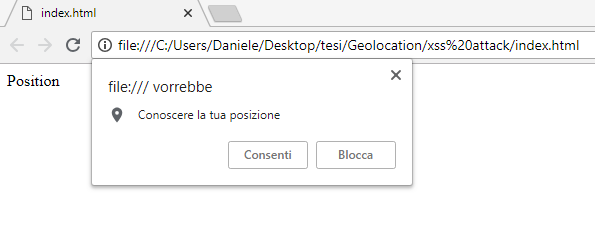
\includegraphics[width=0.5\linewidth]{pos1}
	\caption{Richiesta posizione}
	\label{fig: Richiesta posizione}
\end{figure}
\pagebreak
\\
Supponiamo che un utente malintenzionato abbia avuto modo di inserire una vulnerabilità XSS in un sito Web; tutto ciò che dovra fare è fare in modo che la vittima esegua il seguente codice JavaScript per rubare la posizione.
\lstinputlisting{code/script.js}
Il codice utilizza le proprietà del DOM \textit{cords.latitude} e \textit{cords.langitude} per determinare rispettivamente la latitudine e longitudine, memorizzandole in una variabile, inviandole poi all'attaccante. 
\\
\subsection{Supporto compatibilità web}
\subsubsection{Desktop e mobile}
\begin{figure}[h]
	\centering
	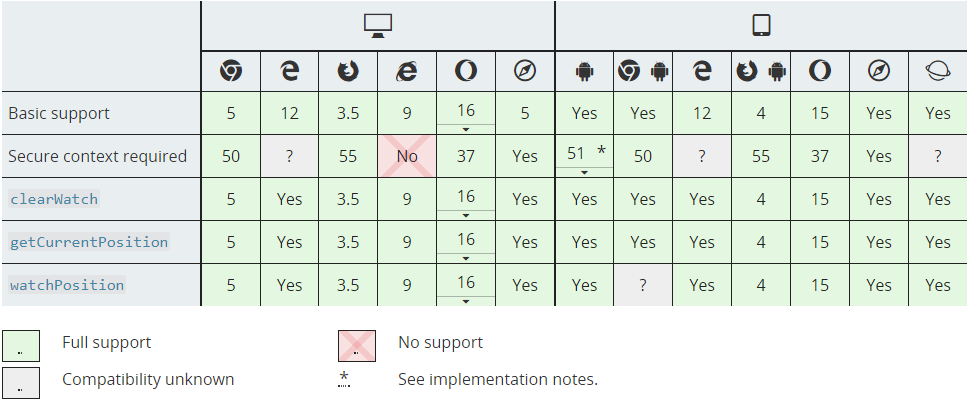
\includegraphics[width=1\linewidth]{compatibility}
	\caption{Compatibilità Desktop e mobile}
	\label{fig: Compatibilità Desktop e mobile}
\end{figure}
\subsection{Conclusioni}
%La Geolocation API è una delle API più semplici.

\newpage
\section{PaymentRequest API}

\subsection{Overview Payment Request}
La PaymentRequest API \cite{rif9} nasce con l'intento di creare esperienze di pagamento semplificate, in quanto ogni sito web ha il proprio sistema di pagamento e molti siti richiedono la ridigitazione manuale delle stesse informazioni più volte, le quali possono essere invece memorizzate e riutilizzate dall'API per completare più rapidamente le transazioni online.

\subsubsection{Vantaggi \cite{rif13}}
\begin{itemize}
	\item \textbf{Esperienza di acquisto rapida:} gli utenti immettono i propri dati una sola volta nel browser, e dopo averli inseriti non è più necessario reinserirli su siti diversi;
	\item \textbf{Esperienza coerente su ogni sito che supporta l'API:} poiché la pagina di pagamento è controllata dal browser si può personalizzare l'esperienza utente, ad esempio includendo la localizzazione per impostare automaticamente la lingua preferita dell'utente o altre features;
	\item \textbf{Gestione delle informazioni:} gli utenti possono gestire le loro carte di credito e gli indirizzi di spedizione direttamente nel browser. Un browser può anche sincronizzare queste informazioni tra dispositivi, rendendo più semplice per gli utenti passare dal desktop al cellulare e viceversa quando si acquistano oggetti;
	\item \textbf{Gestione coerente degli errori:} il browser può controllare la validità dei numeri delle carte e può comunicare all'utente se una carta è scaduta o sta per scadere, può suggerire automaticamente quale carta utilizzare in base ai modelli di utilizzo passati o alle restrizioni del commerciante, o consentire all'utente di dire quale sia la carta predefinita/preferita;
	\item \textbf{Esperienza utente migliorata:} coerenza tra i siti Web, tra browser e sistemi operativi e nuove funzionalità del browser per semplificare il checkout, ecc;
	\item \textbf{Miglioramento della sicurezza:} la PaymentRequest API ha il potenziale per ridurre le opportunità di frode e può facilitare l'adozione di metodi di pagamento più sicuri. Purtroppo ci sono dei problemi di sicurezza analizzati al capitolo 4; 
	\item \textbf{Responsabilità inferiore:} in passato, per creare un'esperienza utente semplificata, i commercianti dovevano memorizzare le credenziali di pagamento degli utenti. Questo non è più necessario, il che può aiutare a ridurre la responsabilità del commerciante nei confronti del cliente.
\end{itemize}

\subsubsection{Come funziona}	
La PaymentRequest API consente a un utente di completare una transazione più facilmente riutilizzando le informazioni memorizzate nel browser o in app di pagamento di terze parti.
Quando l'utente preme un pulsante in una pagina di checkout collegata all'API il commerciante utilizza l'API per richiedere il pagamento. Il commerciante fornisce informazioni su prezzo, valuta e un elenco di metodi di pagamento accettati, e può inoltre richiedere al browser di creare un'interfaccia utente semplificata per raccogliere l'indirizzo di spedizione, le informazioni di contatto e altri elementi all'utente.
Il browser determina quali metodi di pagamento sono supportati dal commerciante tra le varie "app di pagamento" mostrandole all'utente. 
L'utente seleziona un'app di pagamento con la quale pagare, la quale può comportare ulteriori interazioni con l'utente (ad esempio per l'autenticazione). 
Al completamento l'app di pagamento restituisce i dati tramite l'API al commerciante.

\begin{figure}[h]
	\centering
	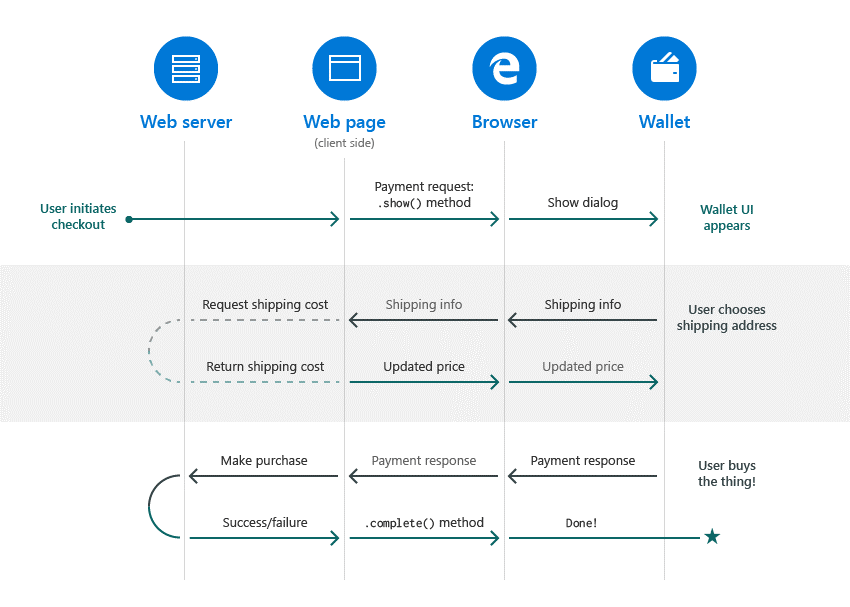
\includegraphics[width=1\linewidth]{SchemaPayment}
	\caption{Schema Payment Request API \cite{rif17}}
	\label{fig:Schema Payment}
\end{figure}
\pagebreak

\subsubsection{Uso API}
\textbf{Ruolo dell'utente}
\\
Gli utenti beneficiano del riutilizzo delle informazioni inserite nel browser o nelle app di pagamento. Quindi, quando si visita un sito Web che sfrutta la PaymentRequest API gli utenti avranno l'opportunità di sfruttare il riutilizzo semplificato delle informazioni archiviate.
\\
\textbf{Ruolo del commerciante}
\\
L'API influisce sul front end (l'interfaccia dell'esperienza utente) e non sul back-end, pertanto il commerciante non dovrebbe dover apportare modifiche all'elaborazione back-end dei vari metodi di pagamento; questo sarà compito del fornitore della pagina di pagamento il quale sostituirà i moduli Web con le chiamate alla PaymentRequest API.
\\
\textbf{Ruolo del browser}
\\
Il browser svolge diversi ruoli:
\begin{itemize}
	\item Calcola l'intersezione dei metodi di pagamento accettati dal commerciante e registrati dall'utente;
	\item Visualizza l'interfaccia utente che consente all'utente di inserire le proprie informazioni;
	\item Funge da canale per i dati da e verso il commerciante e da e verso l'utente.
\end{itemize}
%\textbf{Metodi di pagamento}
%\\
%La PaymentRequest API è progettata per funzionare con un gran numero di metodi di pagamento, i quali vengono identificati attraverso due strade:
%\begin{itemize}
%	\item I metodi di pagamento definiti da W3C sono identificati come "basic-card" e sono composti da stringhe corte;
%	\item I metodi di pagamento definiti da altre parti sono identificati dagli URL.
%\end{itemize}
\textbf{App di pagamento}
\\
La PaymentRequest API determina se un'app di pagamento "corrisponde" a una determinata transazione definendo un algoritmo che considera i metodi di pagamento accettati dal commerciante, dichiarati attraverso un elenco di identificativi del metodo di pagamento, passati attraverso l'API.
Al fine di proteggere la privacy degli utenti i commercianti hanno accesso a informazioni molto limitate dell'utente. 

Vediamo in che modo la PaymentRequest API influisce sul flusso dei metodi di pagamento che già supporta. Il normale flusso per gli utenti di solito implica qualcosa del genere:
\begin{itemize}
	\item Scansione di un elenco di metodi di pagamento accettati;
	\item Scelta di un metodo;
	\item Per i metodi di pagamento che prevedono il lancio di un'app o la visita a un sito Web si invia l'utente a quell'app o sito;
	\item Pagamento completato.
\end{itemize}
La PaymentRequest API consente un flusso migliorato:
\begin{itemize}
	\item L'utente preme un pulsante di acquisto singolo;
	\item Il browser visualizza le app di pagamento dell'utente che possono essere utilizzate per la transazione, ed è probabile che i browser supportino le preferenze dell'utente in modo che un'app di pagamento venga avviata automaticamente su un determinato sito Web, semplificando il checkout.
	\item Per i metodi di pagamento che prevedono il lancio di un'app o la visita a un sito Web, inviare l'utente a quell'app o sito; 
	\item Pagamento completato; 
\end{itemize}
\textbf{Differenze tra metodo di pagamento e app di pagamento}
\\
Un'app di pagamento è il software che l'utente utilizza per pagare, la quale può supportare uno o più metodi di pagamento e può essere implementata utilizzando diverse tecnologie. I browser possono anche fungere da app di pagamento, memorizzando le credenziali dell'utente. In generale più app di pagamento possono implementare lo stesso metodo di pagamento. 
Vi sono casi importanti in cui è disponibile una sola app di pagamento autorizzata a supportare un metodo di pagamento, mentre ci sono casi in cui più app di pagamento possono servire diversi metodi di pagamento. In questo caso non è il commerciante che deve preoccuparsi dell'integrazione software, ma deve solamente richiedere le informazioni attraverso la PaymentRequest API.

\subsection{Specifiche}
\subsubsection{Metodi \cite{rif1}}
Per utilizzare l'API lo sviluppatore deve fornire e tenere traccia di una serie di informazioni chiave, le quali vengono passate al costruttore PaymentRequest come argomenti e successivamente utilizzate per aggiornare la richiesta di pagamento visualizzata all'utente. Queste informazioni sono:
\begin{itemize}
	\item \textbf{PaymentMethodData:} rappresenta i metodi di pagamento che il sito supporta;
	\item \textbf{PaymentDetails:} rappresenta i dettagli della transazione. Ciò include il costo totale e facoltativamente un elenco di beni o servizi acquistati, beni materiali, opzioni di spedizione o "modificatori" su come vengono effettuati i pagamenti: ad esempio "se paghi con una carta di credito di tipo X incorre in una tassa di elaborazione di tot";
	\item \textbf{PaymentOptions:} il PaymentOptions viene passato al costruttore PaymentRequest e fornisce informazioni sulla consegna del prodotto: ad esempio per i beni fisici il commerciante avrà bisogno di un indirizzo fisico dove spedire, mentre per i beni digitali e sufficeinte un'e-mail. Una volta che il PaymentRequest è stato costruito viene presentato all'utente finale tramite il metodo show(), il quale ritorna una promise che, una volta che l'utente conferma la richiesta di pagamento, si traduce in una PaymentResponse;
	\item \textbf{PaymentRequest:} la PaymentRequest serve a effettuare una richiesta di pagamento, in genere associata all'avvio di un processo di pagamento da parte dell'utente. La PaymentRequest consente agli sviluppatori di scambiare informazioni con l'user agent mentre l'utente sta fornendo dati in input. Poiché la visualizzazione simultanea di più interfacce PaymentRequest potrebbe confondere l'utente, questa specifica limita lo user agent a visualizzarne uno alla volta tramite il metodo show();
	\item \textbf{PaymentDetailsInit:} Il PaymentDetailsInit viene utilizzato nella costruzione della richiesta di pagamento;
	\item \textbf{PaymentResponse:} un PaymentResponse viene restituito quando un utente ha selezionato un metodo di pagamento e approvato una richiesta di pagamento.
\end{itemize}

\pagebreak
\textbf{PaymentMethodData}
\\
PaymentMethodData \cite{rif11} contiene gli identificativi dei metodi di pagamento accettati dal sito Web e qualsiasi dato specifico del metodo di pagamento associato.
\lstinputlisting{code/PaymentMethodData.js}
\textbf{PaymentDetails}
\\
I details \cite{rif14} contengono informazioni sulla transazione che l'utente è invitato a completare.
\lstinputlisting{code/PaymentDetails.js}
\pagebreak
\textbf{Opzioni di spedizione}
\\
Qui vediamo un esempio di come aggiungere due opzioni di spedizione ai details. \cite{rif16}
\lstinputlisting{code/OpzioniSpedizione.js}

\flushleft\textbf{Modifiche condizionali alla richiesta di pagamento}
\\
Qui vediamo come aggiungere una tassa di elaborazione per l'utilizzo di una carta di credito. Si noti che richiede il ricalcolo del totale.
\lstinputlisting{code/Tassa.js}
\pagebreak
\textbf{PaymentOptions} \\
Options contiene informazioni che lo sviluppatore ha bisogno dall'utente per eseguire il pagamento.
\lstinputlisting{code/PaymentOptions.js}

\textbf{PaymentRequest} \\
Dopo aver raccolto tutti i bit di informazioni prerequisite, ora possiamo costruirne uno PaymentRequest e richiedere che il browser lo presenti all'utente.
\lstinputlisting{code/PaymentRequest.js}


\subsection{Implementazione PaymentRequest API su una pagina d'esempio \cite{rif15}}
\subsubsection{Costruttore}
L'oggetto PaymentRequest è costruito passando i seguenti parametri:
\begin{itemize}
	\item \textbf{methodData:} una serie di identificativi del metodo di pagamento e tutti i dati pertinenti. Un identificativo del metodo di pagamento è una stringa che identifica un metodo di pagamento supportato;
	\item \textbf{details:} contiene le informazioni sulla transazione, come gli elementi pubblicitari in un ordine;
	\item \textbf{options:} contiene informazioni aggiuntive che il Wallet potrebbe dover raccogliere.
\end{itemize}

Nel seguente esempio stiamo consentendo agli utenti di pagare con qualsiasi carta di debito o di credito appartenente alle reti Visa, MasterCard o Amex. L'oggetto details contiene l'importo totale parziale, l'imposta sulle vendite e il totale dovuto; questi dettagli verranno mostrati all'utente nel portafoglio. Bisogna tenere presente che l'API non aggiunge elementi o calcola l'imposta sulle vendite, spetta al commerciante fornire le informazioni corrette. In questo esempio, stiamo vendendo un bene fisico, quindi chiediamo l'indirizzo di spedizione del cliente.
\lstinputlisting{code/Costruttore.js}
\subsubsection{Visualizzazione dell'interfaccia utente, elaborazione del pagamento e visualizzazione dei risultati}
Una volta creato l'oggetto PaymentRequest è possibile attivare il browser per visualizzare il wallet con request.show() \cite{rif12}. 
\begin{figure}[h]
	\centering
	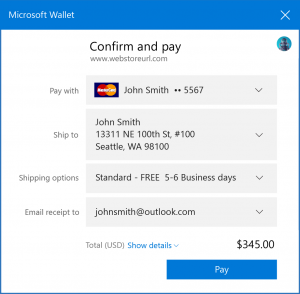
\includegraphics[width=0.5\linewidth]{wallet1}
	\caption{Wallet dopo la chiamata request.show()}
	\label{fig: Wallet dopo la chiamata request.show()}
\end{figure}
\\
\pagebreak
I clienti possono  selezionare le informazioni di pagamento, l'indirizzo di spedizione e altri campi appropriati e cliccare su Paga quando è pronto. A questo punto, gli utenti dovranno verificare la loro identità: in caso di esito positivo verrà soddisfatta la promise request.show() e verranno restituite al sito Web tutte le informazioni che il cliente ha fornito. Per il metodo di pagamento con carta di base l'oggetto risultante conterrà il nome del titolare della carta, il numero della carta, il mese di scadenza e altri campi pertinenti. Il commerciante può quindi utilizzare queste informazioni per elaborare la transazione sul back-end.
Dopo che la risposta è tornata dal server, è possibile utilizzare result.complete('success') per visualizzare la schermata di successo o result.complete('fail') per indicare una transazione fallita.
\lstinputlisting{code/PaymentShow.js}
\pagebreak
Ed ecco i wallet in caso di successo e di fallimento.
\begin{figure}[h]
	\centering
	
\includegraphics[width=0.5\linewidth]{wallet2}
	\caption{Wallet in caso di successo}
	\label{fig: Wallet in caso di successo}
\end{figure}
\begin{figure}[h]
	\centering
	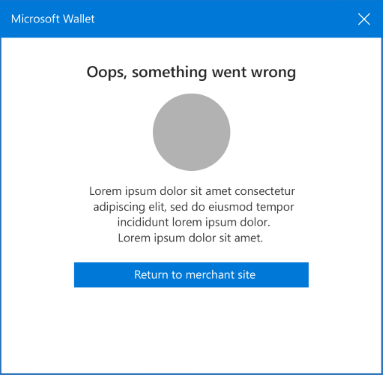
\includegraphics[width=0.5\linewidth]{wallet3}
	\caption{Wallet in caso di fail}
	\label{fig: Wallet in caso di fail}
\end{figure}


\subsection{Rischi e sicurezza \cite{rif19}} 

La PaymentRequest API cerca di garantire la sicurezza dei dati sensibili nei seguenti modi:

\begin{itemize}
\item Per garantire che gli utenti non condividano inavvertitamente informazioni sensibili con una certa origine, l'API richiede che il proprio metodo show() venga attivato solo tramite la volontà da parte dell'utente, ad esempio con un clic. Inoltre, per evitare un'esperienza utente confusa, questa specifica limita la visualizzazione di una finestra alla volta del metodo show() così da non rischiare di inserire dati in più pagine, le quali potrebbero risultare untrusted. 
Se infatti si prova ad aprire più di una finestra dell'API accadrà la seguente situazione:

\begin{figure}[h]
	\centering
	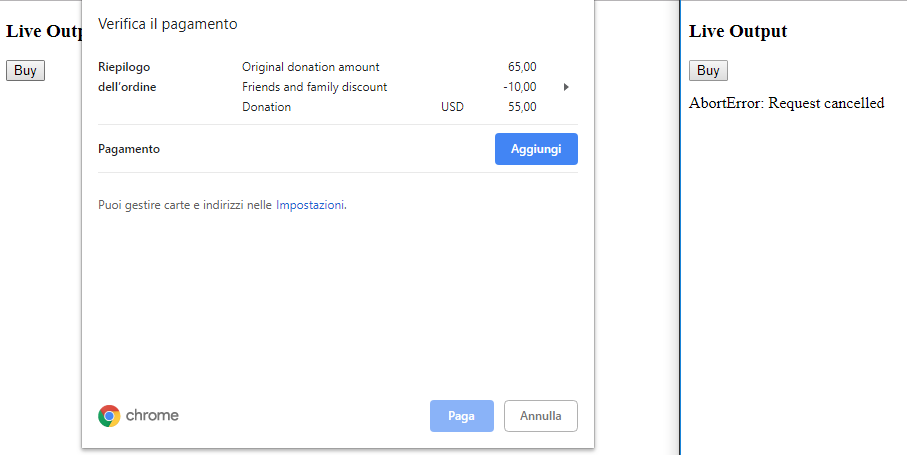
\includegraphics[width=0.5\linewidth]{Buy}
	\caption{Metodo show() richiamato più volte}
	\label{fig: Metodo show() richiamato più volte}
\end{figure}


\item La PaymentRequest API è disponibile solamente su HTTPS, quindi lavora solamente in contesti sicuri per aumentare la sicurezza dell'inserimento delle informazioni. 

\item I commercianti possono delegare la memorizzazione delle informazioni ai fornitori di servizi di pagamento o al browser, senza avere l'onere di memorizzare le informazioni sensibili dell'utente. Inoltre, ovviamente, le informazioni dell'utente non devono essere condivise con uno sviluppatore senza l'autorizzazione dell'utente.
\end{itemize}

Purtroppo un possibile rischio potrebbe essere quello di essere vittima di phishing nel caso fossimo in una pagina untrusted, ovvero viene aperta una pagina identica a quella in cui siamo e tutte le credenziali che inseriamo vengono mandate all'attaccante invece che al sito dove pensiamo di essere. 
Un altro possibile rischio invece potrebbe essere quello di essere vittima di un attacco XSS, ovvero un tipo di attacco nel quale degli script dannosi vengono inseriti lato server all'interno di siti affidabili, dove l'utente è ignaro di questo.
Questo tipo di attacco verrà spiegato nel prossimo paragrafo.

\subsubsection{Esempio di un possibile attacco \cite{rif18}} 
\textbf{Descrizione dell'attacco}
\\
Supponiamo di essere all'interno di un sito affidabile, come Amazon o Facebook, e supponiamo di essere in una pagina di pagamento, come può essere il carrello su Amazon o il pagamento per un'inserzione su Facebook.
Se un attaccante riesce a inserire degli script all'interno di queste pagine riuscirà a ribare le informazioni di pagamento di un utente.
Quando l'utente cliccherà sulla voce "paga", in una delle due piattaforme le quali sono considerate affidabili, verrà eseguito lo script malevolo, invece di quello trusted del sito.
L'utente inserirà tutte le informazioni necessarie al pagamento ma queste verranno mandate e/o visualizzate dall'attaccante.
Come mostrato nell'esempio in figura 14 in questo modo tutte le informazioni possono essere visualizzate dall'attaccante.
Alla richiesta di avvio di un processo di pagamento, ovvero dopo la chiamata al metodo show(), viene creato l'oggetto PaymentRequest nel quale vengono inseriti tutti i dati che l'utente inserisce. 
\begin{figure}[h]
	\centering
	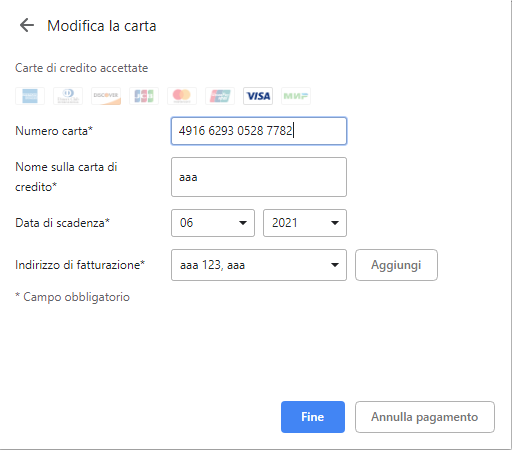
\includegraphics[width=0.5\linewidth]{Chrome1}
	\caption{Inserimento informazioni dell'utente}
	\label{fig: Inserimento informazioni dell'utente}
\end{figure}
\\
\pagebreak
Una volta che l'utente ha approvato una richiesta di pagamento viene restituito un PaymentResponse per approvare tale richiesta. 
\begin{figure}[h]
	\centering
	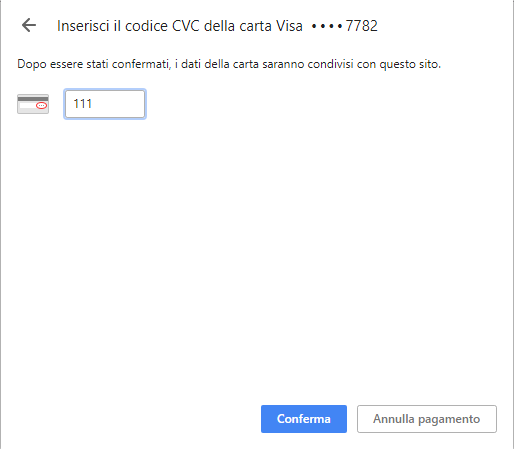
\includegraphics[width=0.5\linewidth]{Chrome2}
	\caption{Inserimento CVV}
	\label{fig: Inserimento CVV}
\end{figure}
\\
\pagebreak
L'oggetto PaymentRequest, creato in precedenza e contenente i dati dell'utente, passa però attraverso il DOM, e quindi può essere intercettato e può essere visualizzato ogni campo inserito dall'utente. Ad esempio nel campo details.cardNumber si può leggere il numero di carta di credito, mentre in details.cardSecurityCode si può leggere il codice CVV; entrambi sono mostrati nell'esempio nella figura seguente.
\begin{figure}[h]
	\centering
	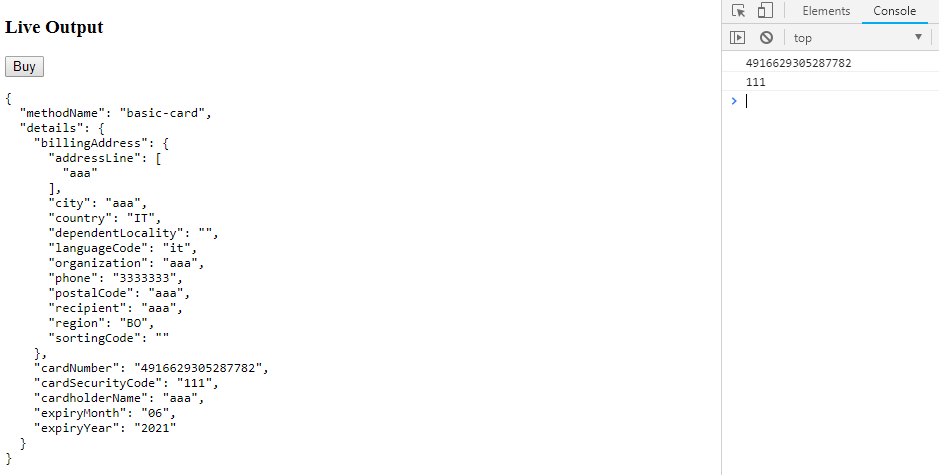
\includegraphics[width=1\linewidth]{Informazioni}
	\caption{Informazioni rubate}
	\label{fig: Informazioni rubate}
\end{figure}
\newpage

\textbf{Come difendersi}

\pagebreak


\subsection{Compatibilità web}
\subsubsection{Desktop}
\begin{figure}[h]
	\centering
	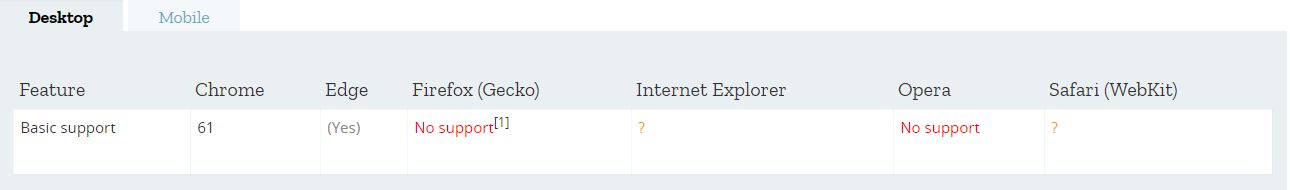
\includegraphics[width=1\linewidth]{Compatibilita1}
	\caption{Compatibilità desktop}
	\label{fig: Compatibilità desktop}
\end{figure}
\subsubsection{Mobile}
\begin{figure}[h]
	\centering
	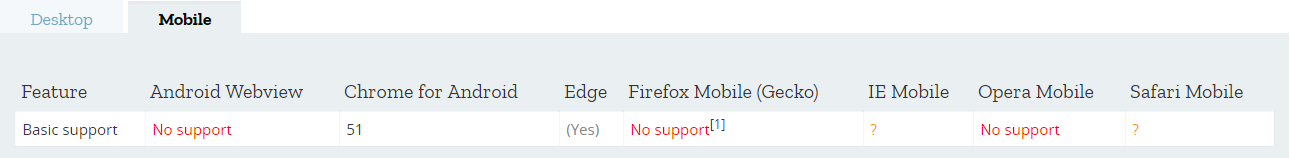
\includegraphics[width=1\linewidth]{Compatibilita2}
	\caption{Compatibilità mobile}
	\label{fig: Compatibilità mobile}
\end{figure}
\subsection{Conclusioni}
La PaymentRequest API è uno strumento per migliorare l'esperienza utente sul Web offrendo ai clienti un'esperienza di acquisto più piacevole, pur avendo delle vulnerabilità. (possono essere colmate?)
\newpage
\cleardoublepage
\section{Service Worker}
\subsection{Overview}
Un ServiceWorker è uno script Javascript che utilizza le Promises per poter eseguire operazioni in modalità asincrona nel browser, avviate in background separato dalla pagina; pertanto non possono modificarne gli elementi del DOM come i normali script ma può comunicare con essi mediante “messaggi”.
Un ServiceWorker si trova tra la nostra applicazione Web e la rete e, come un server proxy, può intercettare tutte le richieste a pagine web e file statici e rispondere secondo politiche che siamo noi stessi a decidere.
I ServiceWorker sono pensati per consentire la creazione di esperienze offline efficaci, intercettare le richieste di rete e intraprendere azioni appropriate in base al fatto che la rete sia disponibile o meno e aggiornare le risorse che risiedono sul server, oltre a consentire l'accesso alle notifiche push e alle API di sincronizzazione in background.
È il browser che in qualsiasi momento deciderà se il ServiceWorker dovrebbe essere o meno in esecuzione così da risparmiare risorse, specialmente sui dispositivi mobili. Per questo può essere che se non facciamo alcuna richiesta HTTP per un certo periodo di tempo o non riceviamo alcuna notifica per un po' è possibile che il browser spenga il Service Worker. Se attiviamo una richiesta HTTP che deve essere gestita dal ServiceWorker il browser la attiverà di nuovo, nel caso in cui non fosse ancora in esecuzione. 

\subsubsection{Impostare i service worker}
Molte funzionalità dei Service Worker oggi sono abilitate di default, ma nel caso non lo fossero bisogna abilitarle nel browser:
\begin{itemize}
	\item Firefox: su \url{about:config} impostare dom.serviceWorkers.enabled su true, riavvia il browser;
	\item Chrome : su \url{chrome://flags} accendere  experimental-web-platform-features, riavvia browser;
	\item Opera : su \url{opera://flags} attivare Support for ServiceWorker, riavvia il browser;
	\item Microsoft Edge : su \url{about:flags} spuntare  Enable service workers, riavvia il browser.
\end{itemize}

\subsubsection{Architettura di base}
Per quanto riguarda i ServiceWorker generalmente vengono eseguiti questi passaggi per l'impostazione di base:
\begin{itemize}
	\item L'URL del ServiceWorker viene recuperato e registrato tramite serviceWorkerContainer.register();
	\item In caso di esito positivo il ServiceWorker viene eseguito in un ServiceWorkerGlobalScope, ovvero un tipo speciale di ServiceContext che scappa dal thread di esecuzione dello script principale senza accesso DOM. Il ServiceWorker ora è pronto per elaborare gli eventi;
	\item L'installazione del ServiceWorker viene tentata quando si accede successivamente alle pagine: un evento di installazione è sempre il primo inviato a un ServiceWorker;
	\item Quando il ServiceWorker è considerato installato il passo successivo è l'attivazione, quindi quando il ServiceWorker è installato riceve un evento di attivazione.
\end{itemize}
\begin{figure}[h]
	\centering
	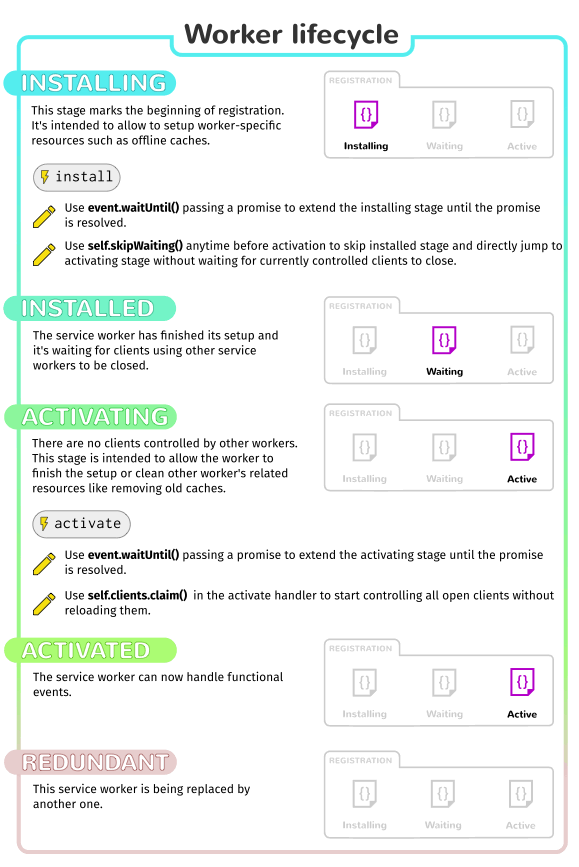
\includegraphics[width=0.6\linewidth]{SwLifecycle}
	\caption{Ciclo di vita del Service Worker}
	\label{fig:Ciclo di vita del Service Worker}
\end{figure}

\subsubsection{Casi d'uso}
I Service Worker sono destinati anche ad altri usi:
\begin{itemize}
	\item Sincronizzazione dei dati in background: viene avviato un Service Worker anche quando nessun utente si trova sul sito, quindi le cache possono essere aggiornate, ecc;
	\item Risposta a richieste di risorse da altre origini;
	\item Caching;
	\item Miglioramenti delle prestazioni, ad esempio prelettura delle risorse che l'utente probabilmente avrà bisogno nel prossimo futuro.
	\item Reagire per inviare messaggi: si può avviare un Service Worker per inviare agli utenti un messaggio per comunicare loro che sono disponibili nuovi contenuti;
	\item Reagendo ad orari e date particolari.
\end{itemize}

\subsection{Ciclo di vita di un Service Worker}
Il ciclo di vita di un service worker è composto da quattro fasi:
\begin{itemize}
	\item Registrazione: il service worker viene scaricato dal browser, analizzato ed eseguito;
	\item Installazione: il service worker viene installato;
	\item Attivazione: il service worker è pronto ed è in grado di poter controllare gli eventi generati dal client;
	\item Fetch: evento generato dal client. Il service worker è in grado di intercettare le richieste e rispondere secondo le opportune strategie di caching. 
\end{itemize}

\subsubsection{Registrazione}

Come prima cosa bisogna comunicare al browser l’esistenza di un ServiceWorker all’interno del sito web. Un Service Worker viene prima registrato utilizzando il metodo ServiceWorker.register() e per farlo basta inserire su tutte le pagine del sito uno script come il seguente:
\lstinputlisting{code/Registrazione.js}
Il codice inizia controllando il supporto da parte del browser verificando la presenza di navigator.serviceWorker. Se supportato, il ServiceWorker viene registrato per mezzo di navigator.serviceWorker.register che restituisce un oggetto Promise il quale si risolve con successo a registrazione avvenuta correttamente.
service-worker.js è il file Javascript residente nella root del sito web e che contiene il codice del service worker, il cui codice è:
\pagebreak
\lstinputlisting{code/Registrazione2.js}
In questo modo viene registrato un ServiceWorker il quale viene semplicemente installato e ad ogni richiesta stampa in console un messaggio con la URL che il browser tenta di scaricare dal server web. Per controllare il caricamento di un Service Worker il codice di questo deve essere eseguito al di fuori delle normali pagine.

Possono esserci diversi motivi per cui il Service Worker non si registra:
\begin{itemize}
	\item Non si sta eseguendo l'applicazione tramite HTTPS;
	\item Il path del Service Worker non è scritto correttamente: deve essere scritto in relazione all'origine, non alla directory radice dell'app;
	\item Il Service Worker a cui ci si riferisce ha un'origine diversa da quella dell'app.
\end{itemize}

\subsubsection{Installazione}
Il ServiceWorker viene scaricato immediatamente quando un utente accede per la prima volta a un sito, o una pagina, controllata dal ServiceWorker, e sarà poi scaricato periodicamente ogni tot periodo di tempo.

L'installazione viene tentata quando il file nuovo che è stato scaricato risulta diverso da un ServiceWorker esistente, o risulta essere diverso dal primo ServiceWorker rilevato per quella pagina/sito. Se è la prima volta che un ServiceWorker viene reso disponibile viene tentata l'installazione e, dopo un'installazione corretta, viene attivato. Se è disponibile un ServiceWorker esistente la nuova versione viene installata in background, ma non ancora attivata; si attiva solo quando non ci sono più pagine caricate che stanno ancora utilizzando il vecchio ServiceWorker. Non appena non ci sono più pagine da caricare il nuovo ServiceWorker si attiva.

Conseguentemente all’installazione viene richiamato l’evento install: tale evento consente di effettuare il precaching, ovvero inserire in cache pagine e file statici del sito web prima di intercettarne le richieste. Per farlo occorre utilizzare gli oggetti Promise event e cache come segue:
\pagebreak
\lstinputlisting{code/Installazione.js}
Se si decidesse di aggiungere/eliminare nuove risorse da inserire in cache bisognerà avere l’accortezza di cambiare il nome della versione del ServiceWorker ed eliminare dalla cache le risorse già presenti.
Una cosa molto importante da sapere è che le risorse da inserire in cache in fase di precaching devono esistere realmente sul server web altrimenti il ServiceWorker genererà un errore fatale e l’installazione non andrà a buon fine. 
Il metodo skipWaiting() consente al ServiceWorker di passare allo stato di attivazione ad installazione conclusa e quindi essere subito operativo.

\subsubsection{Attivazione}
Una volta installato il ServiceWorker passa nello stato di attivazione. Se la pagina al momento è controllata da un altro ServiceWorker quello attuale passa in uno stato di attesa per poi diventare operativo al prossimo caricamento di pagina quando il vecchio ServiceWorker viene sostituito.
Questo per essere sicuri che solo un ServiceWorker (o una sola versione di ServiceWorker) per volta possa essere eseguito nello stesso contesto.
A ServiceWorker attivato viene richiamato l’evento activate, ovvero l'evento per svuotare la cache obsoleta dell’eventuale precedente versione di ServiceWorker. Dopodiché il ServiceWorker sarà in grado di effettuare il fetching di risorse o di restare in attesa di altri eventi.
Di default il nuovo ServiceWorker diventa operativo al refresh della pagina o dopo aver richiamato il metodo clients.claim(); fino a quel momento le eventuali richieste non saranno intercettate. 

\subsubsection{Fetch}
Grazie all’evento fetch il ServiceWorker potrà agire da proxy tra l’applicazione web e la rete.
Il ServiceWorker intercetterà ogni richiesta HTTP del browser e sarà in grado di rispondere a quest’ultimo prendendo la risorsa dalla cache piuttosto che scaricarla dalla rete.
Grazie all’evento fetch il ServiceWorker diventa un vero e proprio strumento per migliorare le performance di caricamento di un sito web.

\subsubsection{Aggiornare il Service Worker}
Se il ServiceWorker è già stato installato ma una nuova versione è disponibile per l'aggiornamento o il caricamento della pagina, la nuova versione viene installata in background ma non sarà ancora attivata. Si attiva solo quando non ci sono più pagine caricate che stanno ancora utilizzando il vecchio servizio. Non appena non ci sono più pagine di questo tipo ancora caricate, il nuovo ServiceWorker si attiverà.

Si dovrà aggiornare il listener install di eventi nel nuovo Service Worker, similmente a questo:
\lstinputlisting{code/Aggiornamento.js}
Mentre accade questo è ancora la versione precedente (v1) quella responsabile per i recuperi, mentre la nuova versione (v2) si sta installando in background.
Quando nessuna pagina sta utilizzando la versione corrente, il nuovo operatore si attiva e diventa responsabile dei recuperi.

\subsubsection{Disintallare il Service Worker}

Rimuovere/disinstallare un ServiceWorker è un’operazione semplice. È possibile eseguirla manualmente dal proprio browser oppure inserendo un semplice script al posto di quello di registrazione del service worker:
\lstinputlisting{code/Disinstallare.js}
Naturalmente è necessario che la pagina contenente il codice di disinstallazione venga visitata dal browser, oppure è possibile rimuovere il ServiceWorker manualmente tramite DevTools.
\newpage
\subsection{Caching}
Diverse sono le strategie che possono essere adottate per migliorare le performance di un sito web mediante i service worker. A seconda del sito e del contesto è possibile adottare una strategia piuttosto che l’altra:
\begin{itemize}
	\item \textbf{Network first} \\
	Questa strategia mira ad avere un contenuto sempre fresco scaricandolo dalla rete, fornendo la copia in cache solo in caso di problemi di connettività, ad esempio in caso di connessione offline;
	\item \textbf{Cache first} \\
	Questa strategia verifica se la risorsa è disponibile in cache: se così fosse viene restituita la copia in cache, in caso contrario la risorsa viene scaricata dalla rete;
	\item \textbf{Network only} \\
	Viene simulato il normale comportamento del browser, ovvero scaricare le risorse direttamente dalla rete;
	\item \textbf{Cache only} \\
	In questo caso il Service Worker risponde solo con elementi conservati in cache: in caso di miss la risposta restituita al browser simulerà l’errore di connessione;
	\item \textbf{Fastest} \\
	Questa strategia mira a fornire all’utente la risposta più veloce: il Service Worker avvia contemporaneamente una richiesta in cache ed una in rete e la prima che risponde verrà restituita all’utente.
	Questa soluzione può essere l’ideale per quei dispositivi con vecchi hard drive dove la lettura da disco può  rivelarsi più lenta del fetch dalla rete, mentre per i dispositivi moderni è meglio utilizzare la strategia cache then network.
	\item \textbf{Cache then network} \\
	Questa strategia mira a fornire il contenuto dalla cache per una risposta molto rapida avviando una richiesta in rete scaricando una copia aggiornata della risorsa e sostituendola con quella in cache; la risorsa ricevuta dalla rete viene poi sostituita con quella presente sulla pagina.
\end{itemize}
È importante sottolineare che il ServiceWorker non utilizza cache a meno che non siamo noi a dirlo, quindi di default il comportamento nella fase di fetch delle risorse sarà quello nativo del browser.

\begin{comment}
Di seguito l’elenco completo delle strategie con esempi di codice di implementazione. 
\subsubsection{Network first}
Questa strategia mira ad avere un contenuto sempre fresco scaricandolo dalla rete, fornendo la copia in cache solo in caso di problemi di connettività (ad esempio in caso di connessione offline).
\lstinputlisting{code/Networkfirst1.js}
Una modifica interessante in questo caso potrebbe essere quella di aggiornare la copia in cache quando la risorsa viene scaricata dalla rete, cosicché in caso di errori di connessione viene restituita la copia più giovane.
\lstinputlisting{code/Networkfirst2.js}
\begin{figure}[h]
	\centering
	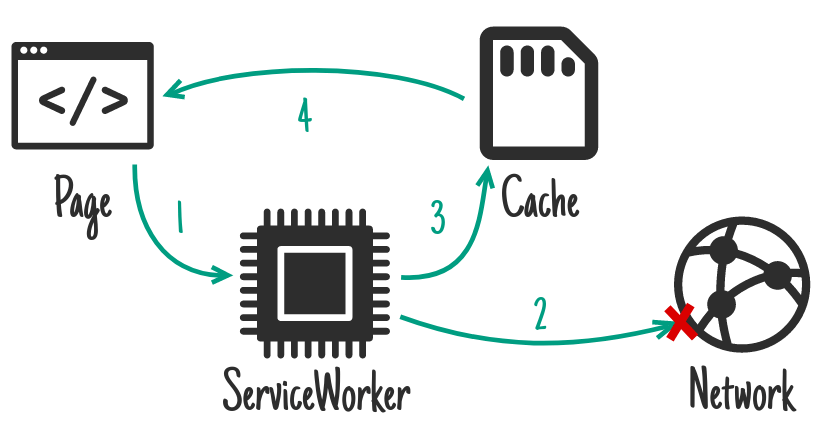
\includegraphics[width=0.7\linewidth]{Strategia1}
	\caption{Network first}
	\label{fig: Network first}
\end{figure}
\subsubsection{Cache first}
Chiamata anche cache, falling back to network, questa strategia verifica se la risorsa è disponibile in cache. Se così fosse viene restituita la copia in cache. In caso contrario la risorsa viene scaricata dalla rete.
\lstinputlisting{code/CacheFirst.js}
\begin{figure}[h]
	\centering
	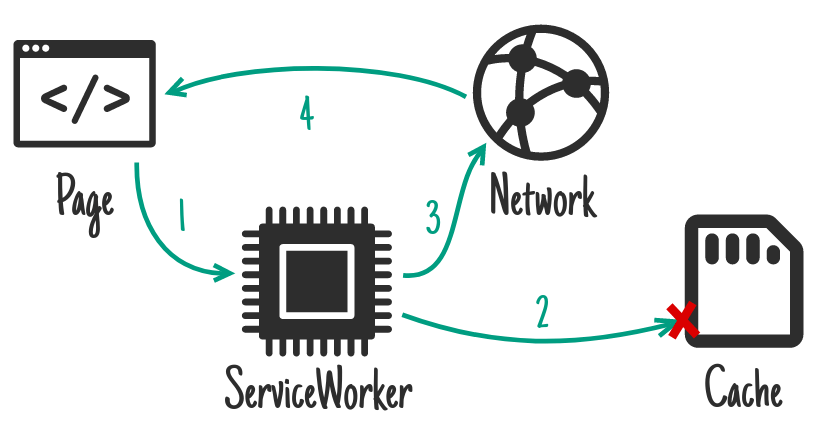
\includegraphics[width=0.7\linewidth]{Strategia2}
	\caption{Cache First}
	\label{fig: Cache First}
\end{figure}
\subsubsection{Network only}
È la strategia più banale in quanto viene simulato il normale comportamento del browser, ovvero scaricare le risorse direttamente dalla rete.

Per applicare  questa strategia basta non inserire alcuna riga di codice all’interno dell’evento fetch:
\lstinputlisting{code/NetworkOnly1.js}
o al limite inserire semplicemente la seguente riga:
\lstinputlisting{code/NetworkOnly2.js}
\begin{figure}[h]
	\centering
	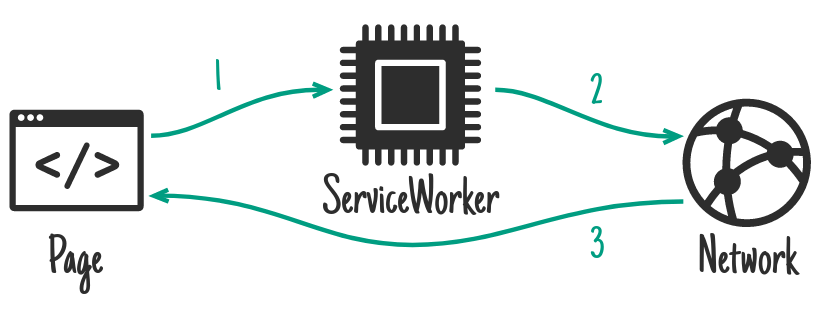
\includegraphics[width=0.7\linewidth]{Strategia3}
	\caption{Network only}
	\label{fig: Network only}
\end{figure}
\pagebreak
\subsubsection{Cache only}
Esattamente opposta alla strategia network only, in questo caso il service worker risponde solo con elementi conservati in cache. In caso di miss la risposta restituita al browser simulerà l’errore di connessione.
\lstinputlisting{code/CacheOnly.js}
\begin{figure}[h]
	\centering
	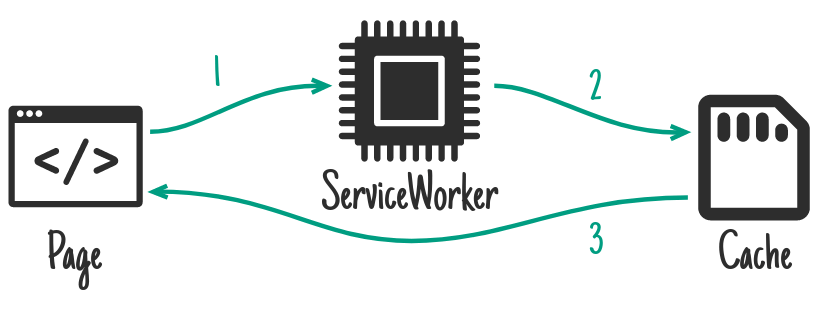
\includegraphics[width=0.7\linewidth]{Strategia4}
	\caption{Cache Only}
	\label{fig: Cache Only}
\end{figure}
\subsubsection{Fastest}
Questa strategia mira a fornire all’utente la risposta più veloce. Il ServiceWorker avvia contemporaneamente una richiesta in cache ed una in rete. La prima che risponde verrà restituita all’utente.
Questa soluzione può essere l’ideale per quei dispositivi con vecchi hard drive dove la lettura da disco può addirittura rivelarsi più lenta del fetch dalla rete. Per i dispositivi moderni è meglio utilizzare la strategia cache then network.
Siccome il ServiceWorker può ritornare un solo Promise, occorre realizzare una funzione a cui passare un array di oggetti Promise, in questo caso cache e fetch, e risolverli quasi contemporaneamente ritornando quello che si risolve per primo.
\pagebreak
\lstinputlisting{code/Fastest.js}
\begin{figure}[h]
	\centering
	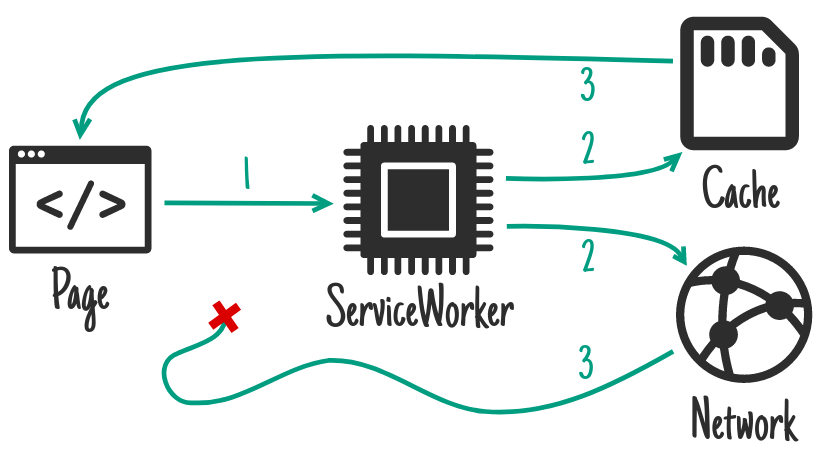
\includegraphics[width=0.7\linewidth]{Strategia5}
	\caption{Fastest}
	\label{fig: Fastest}
\end{figure}
\subsubsection{Cache then network}
Questa strategia mira a fornire il contenuto dalla cache per una risposta molto rapida. Dopodiché in parallelo si avvia una richiesta in rete per scaricare una copia aggiornata della risorsa e sostituirla con quella in cache. La risorsa ricevuta dalla rete viene poi sostituita con quella presente sulla pagina.
Per ottenere questo obiettivo occorre avere sia codice lato pagina che lato ServiceWorker. Questo perché il ServiceWorker deve rispondere subito e non può attendere il completamento di un secondo task senza rallentare l’intera operazione.
Per ottenere qualcosa di analogo usando il solo ServiceWorker occorre utilizzare postMessage affinché la pagina comunichi al service worker la risorsa da interpellare con un secondo fetch, sia esso dalla cache o dalla rete. La complessità rimane uguale ma molto utile in caso si utilizzi il service worker per fare page caching.
\begin{figure}[h]
	\centering
	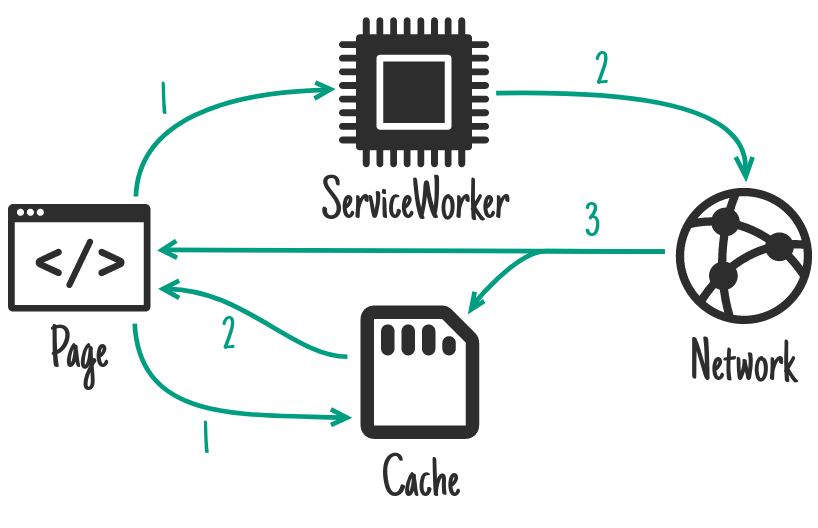
\includegraphics[width=0.7\linewidth]{Strategia6}
	\caption{Cache then Network}
	\label{fig: Cache then Network}
\end{figure}
\end{comment}
\newpage
\subsection{Rischi e sicurezza}
Come già detto i Service Worker operano solo in contesti protetti, ma questo non vuol dire che l'ambiente sia sicuro al 100\% in quanto un ServiceWorker ha la possibilità di importare script da qualsiasi altra origine tramite la chiamata a importScripts, aumentando la capacità di un attaccante XSS di inserire il proprio codice javascript all'interno della pagina, potendo cosi rubare informazioni dell'utente, ad esempio all'inserimento di username e password in una data pagina e portarle fuori. La registrazione dei Service Worker specifica che essi devono essere eseguiti nella stessa origine dei loro chiamanti; il confronto dell'origine è una corrispondenza col prefisso più lungo degli URL serializzati compreso il percorso, quindi ad esempio https://example.com è differente da https://example.com.evil.com. Quindi un attaccante può effettivamente registrare un Service Worker malevolo. Per mitigare questo rischio il browser richiede che l'URL di registrazione del Service Worker provenga dall'origine stessa; quindi per registrare un Service Worker malevolo attraverso un attacco XSS l'utente malintenzionato ha bisogno di ospitare i propri script sul server.
\\
Un possibile scenario potrebbe essere questo: se la pagina ha una vulnerabilità XSS ha anche un endpoint JSONP \footnote{Utilizzato per richiedere dati da un server che risiede in un dominio diverso da quello del client; consente la condivisione dei dati aggirando la politica della stessa origine} e l'utente malintenzionato potrebbe utilizzarlo per:
\begin{itemize}
	\item bypassare CSP\footnote{Cryptographic Service Provider, libreria software sviluppata da Microsoft};
	\item registrare un Service Worker; 
	\item chiamare importScripts per importare uno script malevolo da terze parti.
\end{itemize}
In una situazione XSS del genere il limite della direttiva cache di 24 ore garantisce che un Service Worker malevolo o compromesso sopravviverà a un massimo di 24 ore, o meno in base a come è impostato il sito. Una possibile mitigazione del problema potrebbe essere accorciare la vita dei Service Worker, ovviamente in modo ragionevole altrimenti non sarebbero sfruttate le potenzialità.
\\
Inoltre un Service Worker potrebbe non essere usato solamente per il caching, migliorando i tempi di risposta dell'applicazione o del sito, ma potrebbe anche essere usato per intercettare messaggi, modificandoli e restituendoli errati similmente a man-in-the-middle, come viene mostrato nell'esempio al paragrafo seguente.


- Pro: - VEDERE SE I SW POSSONO MIGLIORARE LA SICUREZZA DI UNA PAGINA, SENZA ESSERE USATI SOLO PER FARE CACHING -
\newpage
\subsection{Esempio di attacco}
Supponiamo di avere questa pagina HTML che carica uno script per l'installazione di un Service Worker, pensando sia sicuro.
\lstinputlisting{code/index.html}
Il file script.js sarà il seguente:
\lstinputlisting{code/scriptSW.js}
\pagebreak
Mentre hack.js, che intercetta ogni richiesta, sarà questo:
\lstinputlisting{code/hack.js}
Infine il file che installerà il Service Worker malevolo sarà questo:
\lstinputlisting{code/install.js}
Ogni richiesta che verrà fatta sarà intercettata dal Service Worker (in questo esempio verrà mostrato il messaggio "Intercepted" nella pagina we ma ovviamente un Web Attacker potrebbe intercettare queste richieste per fare danni --- SISTEMA ---- ) fino a che non sarà disinstallato e non verrà cancellata la cache.
\begin{figure}[h]
	\centering
	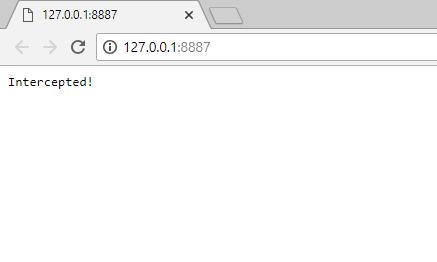
\includegraphics[width=0.7\linewidth]{Intercepted}
	\caption{Intercepted}
	\label{fig: Intercepted}
\end{figure}

\newpage
\subsection{Compatibilità web}
\subsubsection{Desktop}
\begin{figure}[h]
	\centering
	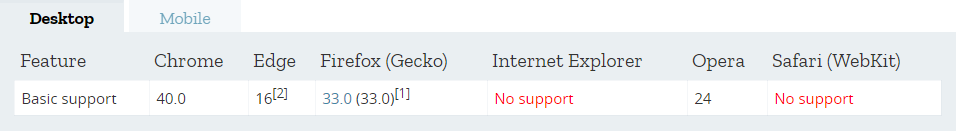
\includegraphics[width=1\linewidth]{CompWeb}
	\caption{Compatibilità web}
	\label{fig:Compatibilità web}
\end{figure}
\subsubsection{Mobile}
\begin{figure}[h]
	\centering
	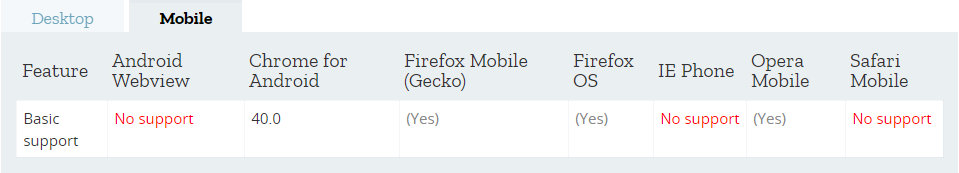
\includegraphics[width=1\linewidth]{CompMobile}
	\caption{Compatibilità mobile}
	\label{fig:Compatibilità mobile}
\end{figure}
\subsection{Conclusioni}
Se realizzati per fare caching i Service Worker possono rendere la navigazione del sito web o dell'applicazione molto più veloce, senza rendere necessarie modifiche al sito o all'applicazione per raggiungere questo scopo. 
Purtroppo sono uno potente strumento anche per scopi malevoli, come illustrato al punto 4.4.
\newpage
\cleardoublepage
\section{Conclusioni}
La tesi ha mostrato come vi siano delle vulnerabilità nelle API web, prendendo un piccolo set di tre API, specificando per ognuna in modo approfondito una spiegazione generale, la sua struttura ed esempi pratici sui problemi di sicurezza e privacy.
-> finire 

\cleardoublepage
\listoffigures
\cleardoublepage
\section{Sitografia}	

\bibliography{Referenze}
\begin{thebibliography}{99}

	%service worker
	
	\bibitem{}
	Angular University (),
	\emph{Service Workers - Practical Guided Introduction (several examples)},
	\url{https://blog.angular-university.io/service-workers/}
	
	\bibitem{}
	formatkaka, mfuji09, Jakubem, MichelleKwa12, Adrianjewell91, KateSturmey, tocretpa, danielpox, jpmedley, chrisdavidmills, akshayjai1, dchest, Sebastianz, neonstalwart, jaffathecake, mouki, Sheppy, Zanadar, fbender, DavidWalsh, fscholz, Heydon, teoli, rassoodock, Meggin (2018),
	\emph{Service Worker API},
	\url{https://developer.mozilla.org/en-US/docs/Web/API/Service_Worker_API}
	
	\bibitem{}
	Throne3d, SphinxKnight, jcsahnwaldt, zekrom-vale, fscholz, arvindpdmn, Jiang-Xuan, wbamberg, schalkneethling, b2397, ramsunvtech, Jedipedia, khaled-hossain-code, mzur, anpa, armujahid, zeevmoney, Vectaio, parambirs, JonathanPool, rwaldron, 6112, kushdilip, thenable, hweeks, Jib, rousan, destin.moulton, Soupedenuit, teoli, ZeroUnderscoreOu, stephaniehobson, psl646, fbergr, atpollmann, kberov, jdsjs, booc0mtaco, programmer5000, otherrealm, kdex, CaemU, Granjow, david-mark, abeltanjq, fredmarques, torazaburo, halfzebra, natoen, tarungarg546, vladan1, igniteram, akshatkedia, nathanh, drostie, mamal, fearlessfool, MiLeung, PeteDevoy, RuiBottoFigueira, JonathanWatt, benjamingr, peter.kehl, ole, jacksonrayhamilton, arai, jmrog, jmsbrr, hltbra, jordanluyke, Sheppy, deisner, kamoroso94, dbruant, mdvorak, kristopolous@yahoo.com, pasqLisena, dstorey, bryanrsmith, nalindak, mattclaw, bitzstein, bgdavidx, Sebastianz, neeraj07rathi, kavitshah8, aochagavia, chrisdavidmills, Goldenyz, jpmedley, hexalys, Callmenorm, vinaygopinath, gaspard, slofurno, Jeremie, fkling42, zbuc, skeller88, miller.augusto, astorije, markg, jucrouzet, Delapouite, Gutworth, realityking, Chudesnov, Account, Fantasyshao, deltab., samvermillion, mnoorenberghe, jsantell, dentuzhik, Irving.Reid, Havvy, hthetiot, wesj, Olafk, DomenicDenicola
	\emph{Promise, Mozilla Developer}
	\url{https://developer.mozilla.org/en-US/docs/Web/JavaScript/Reference/Global_Objects/Promise}
	
	\bibitem{}
	DavidGuan, chrisdavidmills, Deleplace, jwhitlock, simon04, mrmaka, bmihelac, erikadoyle, YoranBrondsema, sideshowbarker, joshua1988, jpmedley, kberov, wbamberg, hl222ih, janx, karolklp, tomayac, maybe, UnJavaScripter, ebidel, JCE, philmander, termosa, franzy1709, stevemao, miguelmota, enguerran, allen.dean, fscholz, Brettz9, jryans, teoli, bhritchie, vrana, rippedspine, adria, Sheppy
	\emph{Using Service Workers, Mozilla Developer},
	\url{https://developer.mozilla.org/en-US/docs/Web/API/Service_Worker_API/Using_Service_Workers}
	
	\bibitem{}
	W3C, Alex Russell, Jungkee Song, Jake Archibald, Marijn Kruisselbrink (2018),
	\emph{Service Workers Nightly},
	\url{https://w3c.github.io/ServiceWorker/}
	
	\bibitem{}
	Mozilla,
	\emph{Service Workers},
	\url{https://serviceworke.rs/}
	
	\bibitem{}
	Google Partners,
	\emph{Tecnologie web avanzate: Service worker},
	\url{https://support.google.com/partners/answer/7336697?hl=it}
	
	\bibitem{}
	Speedy Wordpress,
	\emph{Guida completa ai Service Worker Javascript},
	\url{https://www.speedywordpress.it/guida-completa-ai-service-worker-javascript/}
	
	\bibitem{}
	Matt Gaunt,
	\emph{Service Workers: an Introduction},
	\url{https://developers.google.com/web/fundamentals/primers/service-workers/}
	
	\bibitem{}
	SitePoint,
	\emph{Getting Started with Service Workers},
	\url{https://www.sitepoint.com/getting-started-with-service-workers/}
	
	\bibitem{}
	jakearchibald Github (2017),
	\emph{Service workers explained},
	\url{https://github.com/w3c/ServiceWorker/blob/master/explainer.md}
	
	\bibitem{}
	Lyza Danger Gardner
	\emph{Making A Service Worker: A Case Study}
	\url{https://www.smashingmagazine.com/2016/02/making-a-service-worker/}
	
	\bibitem{}
	Eshun Sharma
	\emph{An Introduction to Service Workers in JavaScript},
	\url{https://codeburst.io/an-introduction-to-service-workers-in-javascript-27d6376460c2}
	
	\bibitem{}
	Nicolas Bevacqua (2015), 
	\emph{Making a Simple Site Work Offline with ServiceWorker},
	\url{https://css-tricks.com/serviceworker-for-offline/}
	
	\bibitem{}
	\emph{Service Worker Security FAQ},
	\url{https://chromium.googlesource.com/chromium/src/+/lkcr/docs/security/service-worker-security-faq.md}
\end{thebibliography}
\end{document}